%%%%%%%%%%%%%%%%%%%%%%%%%%%%%%%%%%%%%%%%%%%%%%%%%%%%%%%%%%%%%%%%%%%%%%%%%%%%%%%%%%%%%%%%%%%%%
%%									Chapitre 1											%
%%%%%%%%%%%%%%%%%%%%%%%%%%%%%%%%%%%%%%%%%%%%%%%%%%%%%%%%%%%%%%%%%%%%%%%%%%%%%%%%%%%%%%%%%%%%%
\chapter{Exploration de l'entreprise}
	\minitoc

%%%%%%%%%%%%%%%%%%%%%%%%%%%%%%%%%%%%%%%%%%%%%%%%%%%%%%%%%%%%%%%%%%%%%%%%%%%%%%%%%%%%%%%%%%%%%




% Début du chapitre

\section{Le rôle du laboratoire Soleil}

	\subsection{Secteur d'activité}
				Le laboratoire SOLEIL est une entreprise du secteur tertiaire. Elle est installé sur le plateau de SAclay en région parisienne. L'objectif du laboratoire est la recherche fondamentale.
				
				Des personnes venant du monde entier viennent faire des recherches au synchrotron SOLEIL parce qu'il y a peu d'équipement aussi performants dans le monde (deux en France). Le second se trouve à Grenoble qui lui est un synchrotron européen donc une partie appartient aux francais et le reste à d'autre pays européen.
	\subsection{Moyens}
		
		\subsubsection{Personnels}
				En décembre 2015, 432 personnes travaillent au laboratoire SOLEIL. L'âge moyen des salariés est de 44 ans. 5 personnes souffrant d'un handicap travaillent à SOLEIL. L'ancienneté moyenne des salariés est de 8 ans.
				
				75\% , c'est à dire 267, des salariés SOLEIL sont des hommes\; 150 sont cadres et 117 sont non cadres.
				
				25\% , donc 80 des personnes embauchées à SOLEIL sont des femmes\; 42 sont cadres et 38 sont non cadres.


		\subsubsection{Équipements}
			
			\paragraph{L'accélérateur d'électrons}
				La plus grande machine du synchrotron SOLEIL est l'accélérateur d'électrons.
				
				L'accélérateur d'électrons permet d'observer de très petites particules grâce à la lumière émise par les électrons.
				
				Un canon, nommé le LINAC, envoie une grande énergie électrique qui va séparer les électrons des atomes. Les électrons sortent du canon à une vitesse de 100 Méga-électrons-Volt.  Dans le booster ils gagnent une énergie de 2750 Méga-électrons-Volt. Quand les électrons ont atteint cette vitesse, ils sont envoyés dans l'anneau de stockage qui est un tube fermé de cinq centimetres de diamètre où ils tournent pendant pusieurs heures à une vitese très proche de celle de la lumière. L'anneau de stockage est constitué d'une succession de parties droites et de virages où les électrons tournent et subissent des accélérations. Quand les électrons tournent ils libèrent des photons, ou lumière. Ce processus est utilisés par 7 lignes de lumières. 21 lignes de lumières utilisent des onduleurs qui accélèrent les électrons qui par la suite libèrent des photons. Ses photons vont être utilisés dans les lignes de lumières, où les scientifiques vont expérimenter la réaction de la lumière sur des objets ou inversement. Les lignes de lumières sont composés de trois cabanes; la cabane optique, la cabane d'expériences et la cabane de vie. Dans la cabane optique on trouve des miroirs déviant la lumière. La cabane d'expériences est l'endroit où on pose l'échantillon a observer et la cabane de vie est l'endroit où on observe l'échantillon et où les scientifiques règlent la caméra. 
			\begin{figure}
 				 \centering
 				 \reflectbox{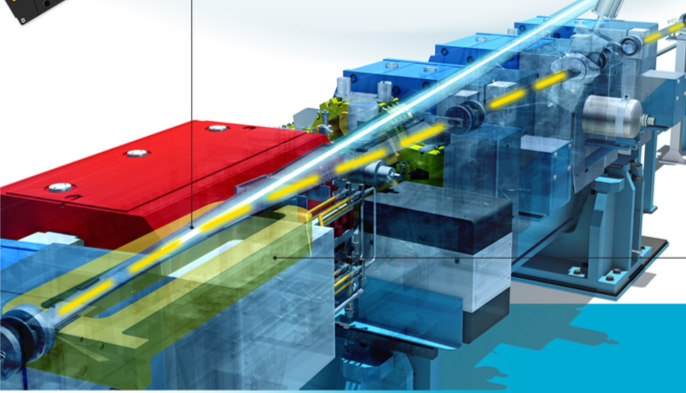
\includegraphics[width=16cm]{Chapitre1/Lesaimants}}
 				 \caption{Les aimants de l'anneau de stockage}
				\end{figure}

			\paragraph{Les Aimants}
				Pour faire tourner les électrons et les garder ensemble, des aimants sont utilisés. Plusieurs sortes d'aimants sont utilisés à SOLEIL. Il y a le dipôle; qui comporte deux aimants et qui fait dévier les éléctrons du côté choisi. Les quadrupôles servent à resserer les éléctrons entre eux parce que quand les éléctrons tournent, ils ont plus de places et donc essaient de s'éloigner car deux charges négatives se rejettent. Les aimants nommés sextupôles font la même chose que les quadrupôles mais plus précisement.Pour alimenter les aimants en éléctricité, on utilise des alimentations. Il existe 32 dipôles, 160 quadripôles et 120 sextupôles au synchrotron SOLEIL. Les dipôles et les quadripôles se situent dans l'anneau de stockage et le booster au contraire des sextupôles qui ne se trouvent que dans l'anneau de stockage. Les dipôles et les quadrupôles sont plus grand dans l'anneau de stockage que dans le booster.

			\paragraph{Autres équipements}
				Le synchrotron SOLEIL possède trois imprimante 3D avec lesquels ils fabriquent de petites pièces. Dans chaque salle on voit un ou plusieurs ordinateurs\; dans la salle de commande, les salles de vie dans les lignes de lumière, les bureaux d'ingénieurs, de dessinateur projecteur, des mécaniciens, des scientifiques... Les aligneurs possèdent des niveaux qui permettent de positionner tous les équipements pour les lignes des lumières, ils utilisent également théodolite, des théodolites améliorés et des lasers trackers plus précis que les deux autres instruments.

				Des pompes sont utilisés par les videurs pour faire le vide dans les tubes de l'accélérateur d'éléctrons.




%\section{Deuxième paragraphe}
%\blindtext

%\bibliographystyle{francaissc}
%\bibliography{Chapitre1/Biblio}